%------------------------------------------------------------------------------------
%	CHAPTER 2
%------------------------------------------------------------------------------------
\chapterimage{headerCap.jpeg}
\chapter{União com C++}

\begin{remark}
	Existem apenas dois tipos de linguagens: aquelas que as pessoas reclamam e as que ninguém mais usa. (Bjarne Stroustrup - Criador da Linguagem C++) 
\end{remark}

\section{Porquê fazer isso?}\index{União com C++}
Talvez a pergunta mais simples seja: O que ganhamos com isso? Fico pensando sinceramente se vale a pena essa união do C++ com o Assembly e a resposta é sempre sim, isso deu muito certo com o ambiente embarcado das placas Arduino e porquê não daria conosco? É verdade que todo casamento tem seus problemas, mas se fosse tudo uma lua-de-mel seria bem esquisito.

Resolvi incluir este capítulo no livro, pois pessoalmente prefiro utilizar o C++ para realizar as entradas e saídas de dados enquanto que o Assembly toda a parte de processamento, ou seja, é aproveitar um melhor de dois mundos. Vejamos como isso funciona e alguns exemplos nas seções seguintes.

\section{Programa 2.1 - Troca de Informações}\index{União com C++}

Diferentemente do que sempre fazemos vamos começar iniciando um programa em C++, chamaremos de "troca.cpp" com o seguinte conteúdo:
\begin{lstlisting}[]
# include <iostream>

using namespace std;

extern "C" int GetValorASM(int a);

int main() {
	cout<<"ASM me deu "<<GetValorASM(32)<<endl;
	return 0;
}
\end{lstlisting}

O comando \textbf{include} indica que iremos trabalhar com uma entrada de dados e a instrução "\textit{using namespace std;}" serve para definir um "espaço para nomes". Isso permite a definição de estruturas, classes e constantes que estão vinculadas para definir funções da biblioteca padrão. 

A instrução que realmente nos interessa é a "extern" que indica o nome de um marcador global que devemos definir, essa recebe um argumento inteiro e retorna também outro. Em linguagens de alto nível sempre temos um ponto de entrada neste caso é o "\textbf{int main()}", neste damos uma saída em cadeia de caracteres para o terminal informando: "ASM me deu " + retorno da chamada \textit{GetValorASM} quando esta recebe 32.

\subsection{Agora sim vamos para o Assembly}\index{União com C++}
Gostaria muito que não se assustasse com o tamanho do programa, pois o mesmo é extremamente pequeno (pensou que ia falar grande?), mas nesse começo quero deixar as coisas simples, crie um programa chamado "troca.asm", com a seguinte codificação:
\begin{lstlisting}[]
section .text

global GetValorASM

GetValorASM:
	mov eax, edi
	add eax, 1
	ret	
\end{lstlisting}

Acredito que nem precise explicar, mas vamos assim mesmo. Antes vamos entender seu fluxo:
\begin{figure}[H]
	\centering
	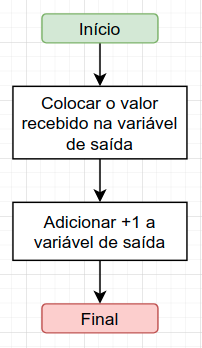
\includegraphics[width=0.25\textwidth]{Pictures/cap02/programa5}
	\caption{Fluxograma do Programa \textbf{Troca de Informações}}
\end{figure}

Primeiro definimos a parte de entrada, não precisamos da sessão .data então vamos direto para a .text porém com uma grande mudança ao invés de definirmos um marcador global "\textit{\_start}" vamos chamar um que o programa C++ está chamando e o definiu "\textit{GetValorASM}" (atenção com as letras maiúsculas ou minúsculas é tudo \textit{case-sensitive}). 

Nesta trecho pegamos o valor do registrador \textbf{EDI} (que é utilizado para a passagem do primeiro parâmetro). Outros registradores utilizados são \textbf{ESI} para o segundo e \textbf{EDX} para o terceiro. Colocamos o valor de \textbf{EDI} em \textbf{EAX} (que é utilizado como valor de retorno da chamada - SEMPRE) e a este adicionamos mais um, ou seja o valor de retorno será sempre o valor de entrada mais um.

\subsection{Modificar o arquivo makefile}\index{União com C++}
Como agora estamos trabalhando com o C++ precisamos realizar uma pequena alteração para o linkeditor, não podemos mais utilizar o \textbf{LD} e devemos passar a utilizar o \textbf{G++}, assim nossa nova codificação para este deve ter o comando: \\
{\ttfamily\$ g++ troca.o troca.cpp -o troca}

Ou seja nosso arquivo agora terá a seguinte codificação:
\begin{lstlisting}[]
NOME = troca

all: $(NOME).cpp $(NOME).o
	g++ $(NOME).o $(NOME).cpp -o $(NOME)
	rm -rf $(NOME).o

%.o: %.asm
	nasm -f elf64 $<	
\end{lstlisting}

Continuamos utilizando o comando \textbf{make} para compilar e linkeditar sem o menor problema e ao executarmos a instrução {\ttfamily ./troca}, teremos como resposta: \\
{\ttfamily\$ ASM me deu 33}

Realmente as coisas estão começando a ficar fáceis demais, e me falaram que o Assembly era difícil.

\section{Programa 2.2 - Questão}\index{União com C++}
Um grande problema que podemos encontrar nessa solução é que agora temos de conhecer a sintaxe de duas linguagens e não apenas de uma e ficamos mais "presos". Porém isso pode ser uma excelente solução na criação de bibliotecas para soluções complexas que envolvem performance de sistemas.

Me perdoe pois aqui devemos pensar de modo simples para sermos didático de modo que possamos compreender na integra como tudo funciona, mas nada impede de alçarmos mais altos voos a partir do que é mostrado aqui.

Novamente vamos começar pelo programa em C++, criamos um arquivo chamado "questao.cpp" com a seguinte codificação:
\begin{lstlisting}[]
#include <iostream>

using namespace std;

extern "C" int Question(int a);

int main() {
  if (Question(27) == 1) {
	cout << "Numero Par" << endl;
  } else {
	cout << "Numero Impar" << endl;
  }
  return 0;
}	
\end{lstlisting}

Nada muito diferente porém no método \textbf{main()} esperamos seja um valor igual a 1 caso o número enviado seja par ou diferente deste caso contrário. Para o programa Assembly que é realmente o que nos interessa, criamos um arquivo chamado "questao.asm" com a seguinte codificação:
\begin{lstlisting}[]
global Question

segment .text

Question:
  mov ebx, edi
  jmp _testar
  ret

_testar:
  cmp ebx, 0
  je _par
  jl _impar
  sub ebx, 2
  jmp _testar	

_par:
  mov eax, 1
  ret

_impar:
  mov eax, 0
  ret
\end{lstlisting}

Conforme definimos no C++ o marcador global chamado é o "Question" que deve estar na nossa seção global, o registrador \textbf{EDI} recebe o parâmetro enviado, agora vamos parar para pensar um pouco (e é isso que amo no Assembly nos força a pensar), quando um número é par? Resposta geral: quando for divisível por 2, correto mas o que isso quer dizer? Resposta geral: quando após a divisão de um número por 2 não restar nada, correto novamente mas então precisamos "transpor" um valor inteiro para um decimal e pegarmos o resto da divisão.

Está vendo com a coisa fica bem complicada? Vamos pensar de modo simplificado, o que vem a seer uma MULTIPLICAÇÃO? É pegarmos o primeiro valor e SOMÁ-LO por ele mesmo quantas vezes indicar o segundo valor. Não é assim que aprendemos lá no primário? Agora a partir desse princípio, o que vem a ser uma DIVISÃO? Ao invés de somar é SUBTRAIR o valor quantas vezes indicar o segundo valor, o resultado é a quantidade de vezes conseguimos fazer isso até um resultado igual a 0. Caso o resultado seja NEGATIVO significa que sobrou um resto. 

Mas o que está nos interessando é se temos um número par ou ímpar, então se o resultado dessa subtração constante por 2 (que seria qualquer número dividido por 2) for 0 significa que este é \textbf{par}, caso contrário menor que 0 ele é \textbf{impar}.

Agora podemos montar nosso fluxograma de acordo com o explicado:
\begin{figure}[H]
	\centering
	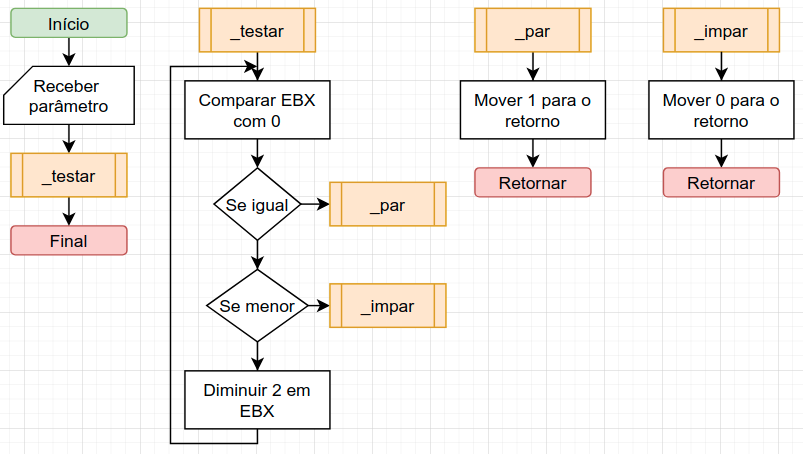
\includegraphics[width=0.8\textwidth]{Pictures/cap02/programa6}
	\caption{Fluxograma do Programa \textbf{Questão}}
\end{figure}

Para compilar e linkeditar copiamos o arquivo makefile indicado anteriormente e mudamos a variável NOME para questao. E podemos modificar o valor do parâmetro passado (que atualmente é 27) para qualquer valor de modo a testarmos as várias possibilidades.

\section{Programa 2.3 - Parâmetros}\index{União com C++}
Nosso próximo programa obterá 3 parâmetros e realizará a soma entre eles, mas como os parâmetros chegam em Assembly? Usamos 3 registradores para isso na seguinte sequência EDI (recebe o 1º parâmetro), ESI (o 2º) e EDX (o 3º). Mas e se tivermos de passar mais que isso? Bem, esse é um dos problemas de utilizar essa forma de programção, nada na vida é infinito.

Vamos começar com a criação de um arquivo chamado "param.cpp", com a seguinte codificação:
\begin{lstlisting}[]
#include <iostream>

using namespace std;

extern "C" int PassarParam(int a, int b, int c);

int main() {
	cout << "Foi retornado:" << PassarParam(50, 40, 10) << endl;
	return 0;
}
\end{lstlisting}

Então temos uma chamada a \textbf{PassarParam} no qual recebe três valores a, b e c do tipo inteiro e esperamos que nos dê o retorno da soma desses. O programa em Assembly será bem simples de se fazer, não pense que aqui guardei algum peguinha para complicar.

Criamos um arquivo chamado "param.asm", com a seguinte codificação:
\begin{lstlisting}[]
global PassarParam

segment .text

PassarParam:
	mov eax, edi
	add eax, esi
	add eax, edx
	ret
\end{lstlisting}

Nada consegue ser mais fácil que isso, colocamos o valor do primeiro parâmetro recebido \textbf{EDI} em \textbf{EAX} (que é o nosso registrador de retorno), em seguida adicionamos o valor de \textbf{ESI} (segundo parâmetro) a \textbf{EAX} e finalmente adicionamos de \textbf{EDX} (terceiro parâmetro) a \textbf{EAX}.

Agora basta copiar o arquivo \textbf{makefile}, alterar o valor da variável NOME e testarmos o programa com a passagem de vários valores.

\section{Programa 2.4 - Fibonacci}\index{União com C++}
O italiano \textit{Leonardo Bigollo Pisano} nos deu uma das mais lindas sequências que é observada constantemente na natureza consiste em uma sucessão de números, tais que, sendo os dois primeiros números da sequência como 1 e 1, os seguintes são obtidos por meio da soma dos antecessores, assim sendo: \\
{\ttfamily 1, 1, 2, 3, 5, 8, 13, 21, 34, ...}
\begin{figure}[H]
	\centering
	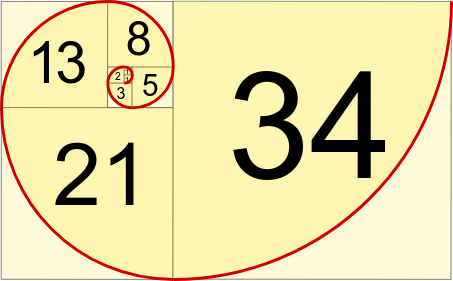
\includegraphics[width=0.35\textwidth]{Pictures/cap02/fibonacci}
	\caption{Sequência de Fibonacci observada na natureza}
\end{figure}

Existem várias aplicações prática para essa sequência (pesquisar, por exemplo, sobre A Identidade de Cassini) mas nosso objetivo aqui é outro, vamos localizar a posição de um determinado elemento dentro dessa sequência, devemos nos ater que a primeira posição é ocupada pelo valor 1, a segunda pelo valor 2, a terceira pelo valor 3, a quarta pelo valor 5, a quinta pelo valor 8 e assim sucessivamente. Deste modo se nosso programa pedir o décimo terceiro valor deve retornar o valor 377, basta fazer as contas.

Vamos começar com a criação do arquivo "fibo.cpp", com a seguinte codificação:
\begin{lstlisting}[]
#include <iostream>

using namespace std;

extern "C" long Fibonacci(long a);

int main() {
  cout << "O " << 13 << " elemento da sequencia de Fibonacci: " << Fibonacci(13) << endl;
  return 0;
}	
\end{lstlisting}

O único detalhe interessante aqui é que ao invés de enviarmos e recebermos um elemento inteiro agora estamos usando um longo (tipo \textbf{long}), e o que isso quer dizer? A quantidade de bits passados e recebidos, um inteiro possui 32 bits de tamanho enquanto que um longo é o dobro, ou seja, 64 bits.

Vamos para a programação Assembly, e começar de modo simples. Criar um arquivo chamado "fibo.cpp" e inserir a seguinte codificação:
\begin{lstlisting}[]
section .text

global Fibonacci

Fibonacci:
  mov eax, 1
  mov r8d, 1
  mov r9d, 1
\end{lstlisting}

Definimos o valor padrão para o registrador de retorno \textbf{EAX}, e populamos os registradores \textbf{R8D} e \textbf{R9D} com os dois primeiros valores da sequencia, e nesses que iremos processar a combinação de sequência.

O cálculo dessa sequência é relativamente simples, porém envolve uma troca de posições, novamente PENSEMOS SIMPLES, temos o seguinte, se o valor pedir 1º elemento, vamos pegar esse valor e diminuir 1 se o resultado for 0 podemos retornar, assim continuamos nosso programa com:
\begin{lstlisting}[]
Calcular:
  sub edi, 1 
  cmp edi, 0
  je Terminar
\end{lstlisting}

Lembre-se que o primeiro parâmetro será enviado em \textbf{EDI}, sendo este será o nosso controlador, se o programa continuar seu fluxo, ou seja não entrar no marcador \textbf{terminar}, realizamos os seguintes movimentos:
\begin{lstlisting}[]
  mov eax, r8d
  add eax, r9d
\end{lstlisting}

Infelizmente não existe um comando para dizer assim: {\ttfamily EAX = R8D + R9D}, então devemos realizar isso de forma "parcelada", primeiro colocamos o valor de \textbf{R8D} em \textbf{EAX} para em seguida somarmos o valor de \textbf{R9D}.

Próximo passo e procedermos a troca, ou seja, andarmos os valores:
\begin{lstlisting}[]
  mov r8d, r9d
  mov r9d, eax
  jmp Calcular
\end{lstlisting}

Colocamos o valor de \textbf{R9D} em \textbf{R8D} e \textbf{EAX} em \textbf{R9D} e saltamos para o marcador \textbf{Calcular} e fazemos novamente todo o processo até que \textbf{EDI} seja 0 e salte para o marcador \textbf{Terminar} com a seguinte codificação.
\begin{lstlisting}[]
Terminar:
  ret	
\end{lstlisting}

Que simplesmente procede o retorno. Um comentário que recebi quando publiquei esse programa: "Pombas você deve ser um PÉSSIMO programador consigo fazer isso com muito menos linhas!". Primeiro que isso não é uma competição, segundo que meu objetivo ao colocar um programa aqui é que o mesmo seja didático e possamos aprender algumas coisas, e terceiro, também consigo programá-lo com menos linhas utilizando apenas os registradores \textbf{EAX} e \textbf{R8D} do seguinte modo:
\begin{lstlisting}[]
section .text

global Fibonacci

Fibonacci:
  mov eax, 1
  mov r8d, 1
Calcular:
  sub edi, 1 
  cmp edi, 0
  je  Terminar
  add eax, r8d
  jmp Calcular

Terminar:
  ret
\end{lstlisting}

Mas deste modo o que teríamos para discutir ou aprender? Pois todos os movimentos já foram vistos anteriormente. O objetivo aqui é aprendermos a programar de um jeito simples e observando os detalhes da linguagem, se deseja aprender \textbf{lógica} lhe recomendo buscar um bom curso ou livro que ensine isso, pois aqui não pretendo ficar preocupado com o perfeccionismo.

\section{Programa 2.5 - Dupla Chamada}\index{União com C++}
Tudo bem até o momento compreendemos que podemos passar valores do C++ para o Assembly, porém com tudo que foi mostrado parece que só podemos ter uma única chamada. Errado podemos ter várias chamadas, inclusive a vários pontos do programa, desde que esses tenham a seguinte característica sejam declarados com o comando \textbf{GLOBAL} e finalizem com o comando \textbf{RET}. 

Vamos pensar em 2 estruturas, primeira:
\begin{lstlisting}[]
int teste1(int valor1, int valor2) {
  if (valor1 > valor2) {
    return valor1;
  } else {
    return valor2;
  }
}
\end{lstlisting}

Uma decisão no qual retorna o valor que for maior entre dois valores passados. E uma segunda estrutura:
\begin{lstlisting}[]
int teste2(int valor1) {
  int ret = 0;
  switch (valor1) {
    case 1:
      ret = 5;
      break;
    case 2:
      ret = 6;
      break;
    case 3:
      ret = 4;
      break;
    case 4:
      ret = 5;
      break;
  }
  return ret;
}
\end{lstlisting}

Nesta escolha caso seja passado o valor 1 retorna 5, caso 2 retorna 6, caso 3 retorna 4, caso 4 retorna 5 e caso contrário o valor padrão 0. Como disse anteriormente não se importe muito com a lógica nesses casos pois é apenas uma exemplificação.

Começamos com a criação do arquivo "decisao.cpp" com a seguinte codificação:
\begin{lstlisting}[]
#include <iostream>

using namespace std;

extern "C" int Teste1(int valor1, int valor2);
extern "C" int Teste2(int valor1);

int main() {
  cout << "Do teste1 foi retornado: " << Teste1(30, 20) << endl;
  cout << "Do teste2 foi retornado: " << Teste2(3) << endl;
  return 0;
}
\end{lstlisting}

Temos a chamada de dois marcadores chamadas Teste1 e Teste2, que farão exatamente o que foi proposto anteriormente. Começamos a montagem do programa "decisao.asm" com a seguinte codificação:
\begin{lstlisting}[]
segment .text

global Teste1
global Teste2
\end{lstlisting}

Ou seja, pouco importa a quantidade de marcadores globais que criemos no programa Assembly desde que todas estejam declaradas no comando GLOBAL. Para o marcador \textbf{Teste1}:
\begin{lstlisting}[]
Teste1:
  cmp edi, esi
  jg voltaEDI
  jmp voltaESI

voltaEDI:
  mov eax, edi
  ret

voltaESI:
  mov eax, esi
  ret
\end{lstlisting}

Comparamos os dois valores passados se o primeiro (\textbf{EDI}) for maior que o segundo retornamos este movendo-o para o registrador de retorno (EAX), caso contrário o segundo (ESI). Para o marcador \textbf{Teste2}:
\begin{lstlisting}[]
Teste2:
  cmp edi, 1
  je volta5
  cmp edi, 2
  je volta6
  cmp edi, 3
  je volta4
  cmp edi, 4
  je volta5
  mov eax, $0x0
  ret

volta4:
  mov eax, $0x4
  ret

volta5:
  mov eax, $0x5
  ret    

volta6:
  mov eax, $0x6
  ret
\end{lstlisting}

Se formos comparar com Teste1 temos apenas uma sequência de comparações e o salto para onde deve ir caso essa comparação seja igual.

Nativamente desta forma em Assembly são transpostos os comandos \textbf{IF} e \textbf{SWITCH} de C, realmente as coisas começam a ficar muito simples.

\section{Acabou?}\index{União com C++}
Esses são os casos mais comuns que utilizamos a programação Assembly em conjunto com o C++ (ou mesmo com outras linguagens de alto nível), porém o objetivo desse livro não é mesclar esse assunto mas o de ensinar a programar em Assembly NASM.

Na próximo capítulo veremos alguns programas para praticarmos um pouco mais nossa lógica de programação juntamente com o Assembly.

% Final do Capítulo
\clearpage